\documentclass[../main.tex]{subfiles}
\graphicspath{{\subfix{../diagrams/}}}

\begin{document}

\section{AlexCore}
Add text here


\subsection{Core Architecture and Pipelines}
AlexCore has five stages; frontend, decode, issue, execute, and commit. Each stage has one pipeline except for the frontend and execute stages each having two pipelines, making a total of seven pipelines.

\subsubsection{Stage details}
\begin{enumerate}
  \item \textbf{Frontend:} \\
  Fetches instructions from memory via the OpenPiton core interface, capable of fetching one instruction per cycle.
 \item \textbf{Decode:}\\
 Decodes fetched instruction and sets control signals accordingly. 
 \item \textbf{Issue:}\\
 Register file and CSR  read and write operations all occur in this stage. This stage also includes the scoreboard, which manages data, control, and memory hazards.\\ The frontend, decode, and issue stages are stalled on hazards.
 \item \textbf{Execute:}\\
This stage includes the ALU, multiplication and division unit, memory controller, CSR unit, exceptions logic, and write-back multiplexer.
 \item \textbf{Commit:}\\
 Contains the write back values to the register file and CSR register file. 
\end{enumerate}

\begin{figure}[bh]
\centering
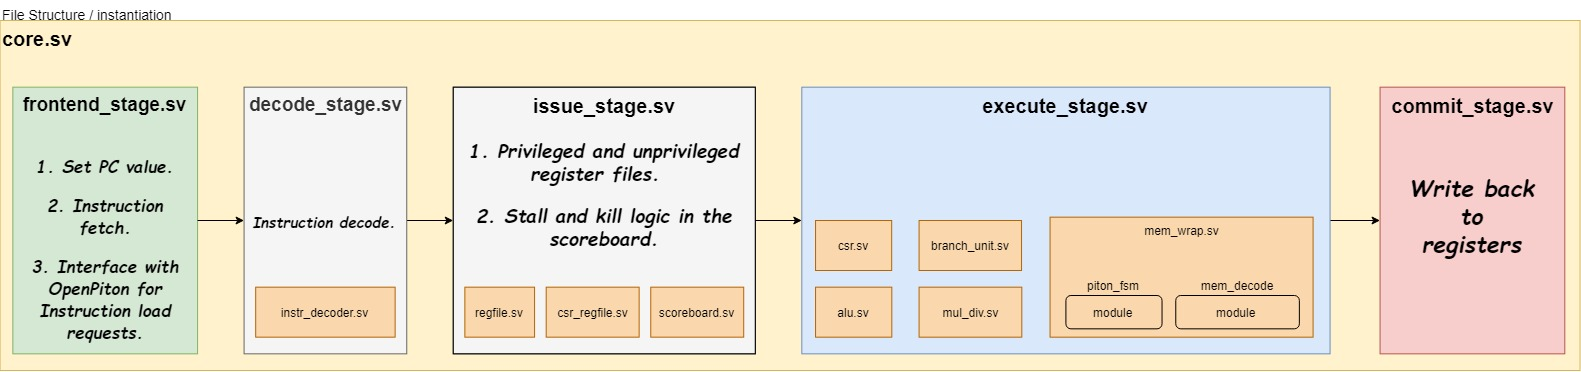
\includegraphics[width=15cm, height=7cm]{diagrams/CoreHirearchy.jpg}

\caption{Core file hirearchy}
\label{fig:files}
\end{figure}

\begin{figure}[p]
\centering
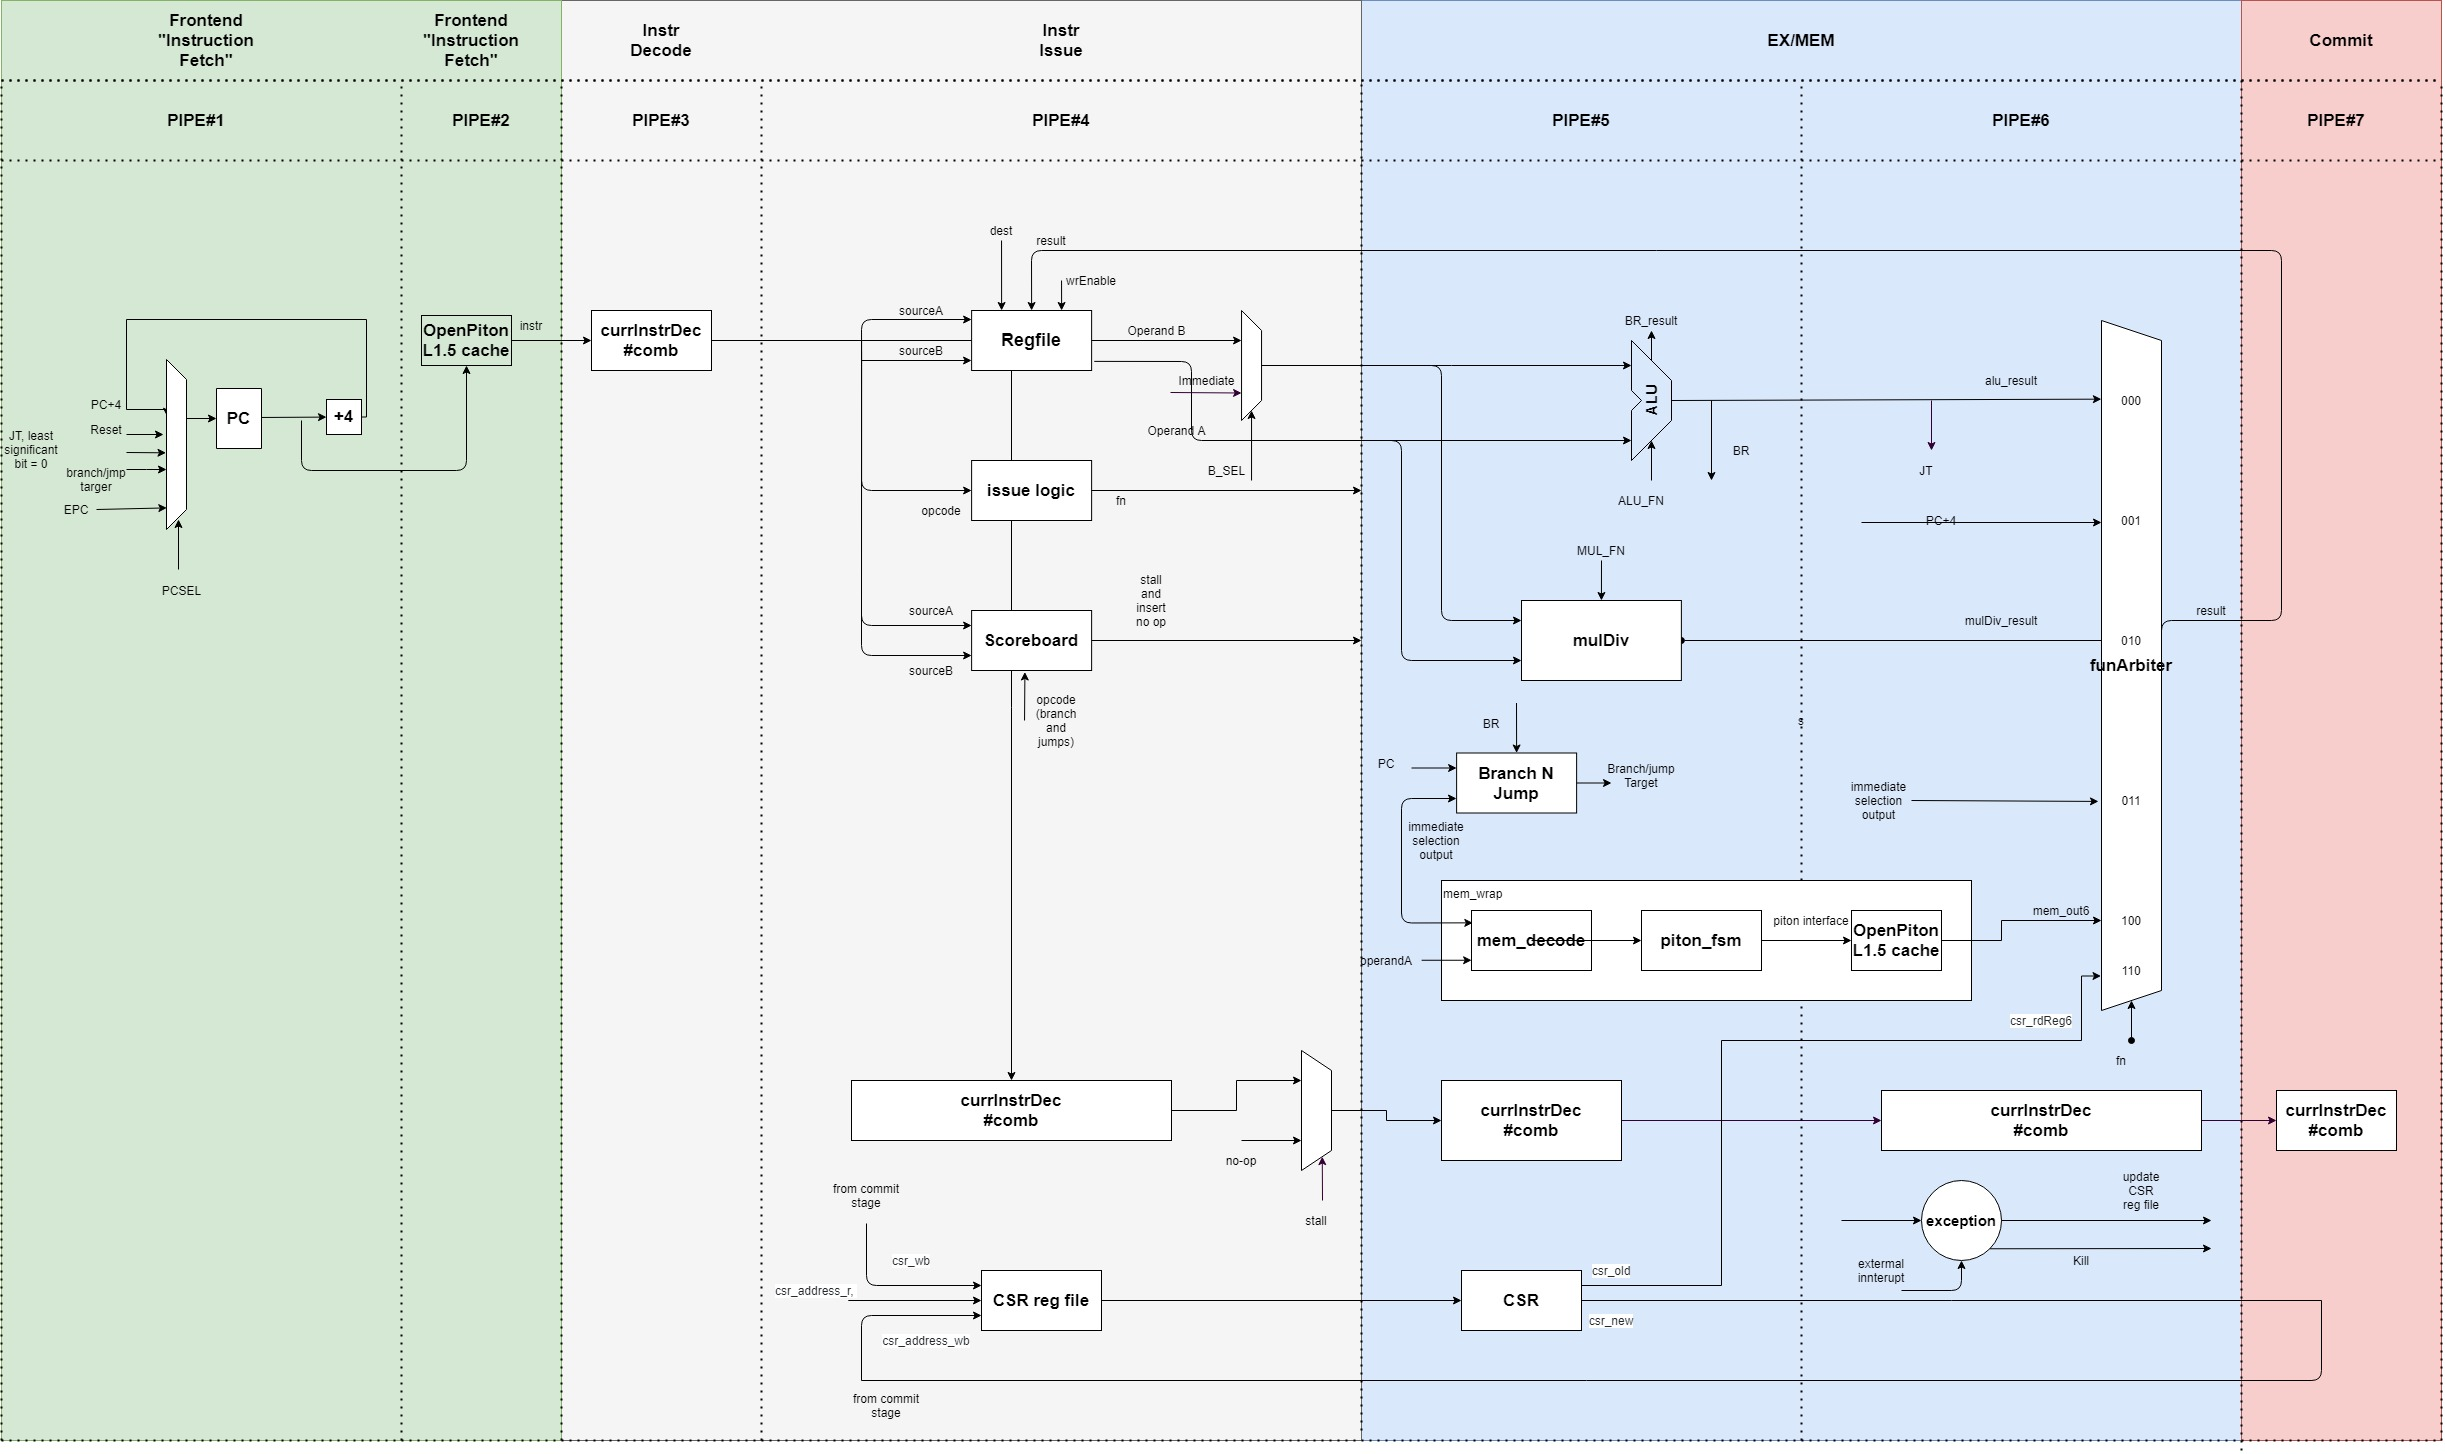
\includegraphics[scale = 0.27,angle = 90]{diagrams/CoreTopLevel.jpg}

\caption{Core Architecture Diagram}
\label{fig:img1}
\end{figure}

\subsection{Arithmetic and Logic Operations}
The execution of these operations is split between two units; ALU, and multiplication and division unit. The ALU executes I-extension operations while the multiplication and division unit executes M-extension operations. The ALU also performs calculation regarding branch operations.

\subsubsection{ALU operations}
The ALU takes the following input signals:
\begin{itemize}
  \item alu\_fn: selects the operation that the ALU will perform. Table \ref{ch4.1} shows the input values corresponding to each operation 
   \item btype: determines that the ALU operation is a branch operation. 
   \item bneq: asserts the branch signal if operandA and operandB are not equal.
  \item operandA: ALU input A.
  \item operandB: ALU input B.
\end{itemize}

\noindent The ALU takes the following output signals:
\begin{itemize}
  \item btaken: Indicates that the branching condition is met.
  \item result: ALU arithmetic and logical operation result output.
\end{itemize}

\begin{table}[h!]
\begin{center}
\begin{tabular}{|c | c|}
    \hline
    alu\_fn & Mnemonic\\
    \hline
    4'b0001 & ADDI, ADD  \\ 
    \hline
	4'b0001 & SLLI, SLL  \\
	\hline
	4'b0010 & SLTI, SLT  \\
	\hline
	4'b0011 & SLTIU, SLTU \\
	\hline
	4'b0100 & XORI, XOR  \\
	\hline
	4'b0101 & SRLI, SRL  \\
	\hline
	4'b0110 & OR, ORI \\ 
	\hline
	4'b0111 & ANDI, AND \\
	\hline
	4'b1000 & SUB \\
	\hline
	4'b1001 & BGE\\  
	\hline
	4'b1010 & BGEU \\ 
	\hline
	4'b1101 & SRAI, SRA \\
	\hline
\end{tabular}
\end{center}
\caption{ALU operations}
\label{ch4.1}
\end{table}

\subsubsection{Multiplication and division operations}
It takes the following input signals:
\begin{itemize}
   \item  mulDiv\_op: selects the operation type. Table \ref{ch4.2} shows the input values corresponding to each operation
   \item a,b: input operands.
\end{itemize}

And res as the output result signal.

\begin{table}[h!]
\begin{center}
\begin{tabular}{|c | c|}
    \hline
    mulDiv\_op & Mnemonic\\
    \hline
    4'b0000 & NoOp  \\ 
    \hline
	4'b0011 & MUL  \\
	\hline
	4'b0101 & MULH  \\
	\hline
	4'b0111 & MULHU \\
	\hline
	4'b0110 & MULHSU  \\
	\hline
	4'b1001 & DIV  \\
	\hline
	4'b1011 & DIVU \\ 
	\hline
	4'b1101 & REM \\
	\hline
	4'b1111 & REMU \\
	\hline
\end{tabular}
\end{center}
\caption{Multiply/divide operations}
\label{ch4.2}
\end{table}

%%%%%%%%%%%%%%%%%%%%%%%%%%%%%%%%%%%%%%%%%%%%%%%%%%%%%%%%%%%%%%%%%
\subsection{Handling Hazards}
Add text here
%%%%%%%%%%%%%%%%%%%%%%%%%%%%%%%%%%%%%%%%%%%%%%%%%%%%%%%%%%%%%%%%%


\end{document}
